% \documentclass[journal]{IEEEtran}
% %

% \usepackage{cite}
% \usepackage{time}
% \usepackage{amsmath}
% \usepackage{graphicx}
% \usepackage{graphics}
% \usepackage{epsfig}
% \usepackage{latexsym}
% \usepackage{amsfonts}
% \usepackage{amssymb}
% \usepackage{paralist}
% \usepackage{xspace}
% \usepackage{mathrsfs}
% \usepackage{psfrag}
% \usepackage{color}
% \usepackage[ruled]{algorithm}
% \usepackage[noend]{algorithmic}
% \usepackage{url}
% \usepackage{subfigure}
% \usepackage{multirow}
% \newtheorem{theorem}{Theorem}
% \newtheorem{axiom}[theorem]{Axiom}
% \newtheorem{corollary}[theorem]{Corollary}
% \newtheorem{conjecture}[theorem]{Conjecture}
% \newtheorem{definition}{Definition}
% \newtheorem{lemma}{Lemma}
% \newtheorem{remark}[theorem]{Remark}
% \newtheorem{proposition}[theorem]{Proposition}

\newcommand{\bin}[1]{{\color{blue} #1}}


% \newcounter{tempcounter}



\documentclass[10pt,journal,compsoc]{IEEEtran}
\usepackage{graphicx}
\usepackage{subfigure}
\usepackage{cite}
\usepackage{epstopdf}
\usepackage{breakurl}
\usepackage[justification=centering]{caption}
\usepackage{amsmath}
\usepackage{color}
\IEEEpubid{\begin{minipage}{\textwidth}\ \\[12pt]
		xxx-x-xxxx-xxxx-08/19/\$31.00 \copyright 2019 IEEE \\
		IEEE Network 
\end{minipage}}

\hyphenation{op-tical net-works semi-conduc-tor}



\begin{document}

%\title{Toward High Performance, Security and Visibility Task Offloading in Drone-aided Mobile Edge Computing}
\title{Blockchain based Task Offloading in Drone-aided Mobile Edge Computing}

\author{Shuyun Luo$^{\star}$, Hang Li$^{\star}$, Zhenyu Wen$^{\dagger \Upsilon}$, Bin Qian$^{\dagger}$, Graham Morgan$^{\dagger}$, Antonella Longo$\ddagger$, Omer Rana$^\&$ and Rajiv Ranjan$^{\dagger}$
        %Deepak Puthal $^{b}$,~\IEEEmembership{Senior Member,~IEEE}, Jian Hou$^{a}$ \\
       % and~Jane~Doe,~\IEEEmembership{Life~Fellow,~IEEE}% <-this % stops a space
     
\small{$^\star$ School of Information Science $\&$ Technology, Zhejiang
Sci-Tech University, Hangzhou, 310018, China}\\
\small{ $^\dagger$ School of Computing, Newcastle University, Newcastle upon Tyne NE1 7RU, U.K.} \\
\small{ $^\&$ School of Computer Science and Informatics, Cardiff University, Cardiff, CF24 3AA} \\
\small{ $^\ddagger$ University of Salento}
\small{ $^\Upsilon$ Zhenyu Wen is the corresponding author}
}


\markboth{Journal of \LaTeX\ Class Files,~Vol.~14, No.~8, August~2015}%
{Shell \MakeLowercase{\textit{et al.}}: Bare Demo of IEEEtran.cls for IEEE Journals}


\maketitle


\begin{abstract}
An increasing number of cloud providers now offer Mobile Edge Computing (MEC) services for their customers to support task offloading. This is undertaken to reduce latency associated with forwarding data from IoT devices owned by customers to cloud platforms. However, two challenges remain in existing MEC scenarios: (i) the coverage of MEC services is limited; (ii) there is limited ability to develop an audit trail about which MEC service providers have processed a user's data. A new architecture for automatically offloading user tasks in MEC scenarios is proposed which addresses the two challenges above. The architecture makes use of drones to dynamically cache data generated from IoT devices and forwards this data to MEC servers that participate in a private blockchain network. We use simulation to demonstrate the use of the proposed architecture in practical MEC scenarios, demonstrating both the efficiency of the task offloading process and greater visibility of MEC service providers involved in processing user data.    

\end{abstract}

% Note that keywords are not normally used for peerreview papers.
\begin{IEEEkeywords}
 Mobile Edge Computing, Drone, Blockchain, Task Offloading
\end{IEEEkeywords}

\IEEEpeerreviewmaketitle
\section{Introduction}
\label{sec:introduction}

% Introduce the main tech of MEC, task offloading, add reference.
With the development of various mission-critical applications of Internet of Things (IoT), e.g. vehicular networks (both vehicle-to-vehicle and vehicle-to-infrastructure), augmented reality and city sensing, there is a need to ensure sufficient computational capacity and low latency connectivity is available for devices that are used in such applications. However, there is a tension between having sufficient computing resource and low latency in IoT applications. A cloud platform can have sufficient computing resources, however transferring data from IoT devices to cloud-based systems may introduce significant delay. This is particularly true in closer proximity to IoT devices, where the first hop network from the IoT device may have limited network capacity. A Mobile Edge Computing (MEC) framework is proposed to address some the above issues by offloading computation from IoT devices to local/ regional MEC servers instead of using a remote cloud system. This overcomes a number of potential constraints in current systems: lower energy consumption at the terminal devices\cite{mach2017mobile}, reduced requirement to transfer security-sensitive data to a cloud platform, and the need for network capacity between the IoT device and the cloud platform (over a multi-hop connection). 

Many existing offloading strategies for MEC environments focus on maximizing applications' performance by partitioning computational tasks across  IoT devices, MEC servers, and a cloud platform. However, there is limited coverage on development of the MEC network itself -- which is often assumed to be made of homogeneous types of devices/ resources. In rural environments and emergency relief scenarios, for example, the number of MEC servers are very limited. As a result, not all IoT devices can be covered by the MEC network. Inspired by~\cite{chen2017caching,zeng2016wireless,jeong2017mobile} that use drones (Unmanned Aerial Vehicles (UAVs)) to cache data generated from IoT devices that cannot be reached by cellular networks, we also describe the use of drones to forward cached data from IoT devices to MEC servers, rather than a  cloud platform.  The aim is to reduce the latency of data transmission via cellular networks.  

In addition, MEC server may be owned and operated by various organizations (e.g. Huawei, Google, Microsoft) and these providers need to work collaboratively to offer the ``best'' service to their costumers. This also raises a significant challenge of how to improve the visibility of the MEC service providers for handling users' sensitive data, or ensure some standard security and privacy requirements such as General Data Protection Regulation (GDPR) are met.  To achieve this, we use a blockchain network to improve the visibility of MEC service providers, helping increase trust from their customers. Moreover, we choose a permissioned, private blockchain to meet two essential requirements of our system: (i) offloading of tasks to the ``best" MEC server; (ii) developing a non-modifiable audit trail of which MEC server has been involved in processing user data (identifying ownership and processing carried by the MEC server). 

In this paper, we present a new secure offloading system that utilizes drones to extend the coverage of MEC networks and a private Blockchain is used to ensure the visibility and accountability of the MEC server providers on operating users' data while guaranteeing the performance of each offloading task. The proposed system has the following advantages:

% To tackle the above issues of task offloading in MEC scenarios, we present a high reliable architecture with drones based on the smart contract, shown in Figure \ref{fig:network-arch}, which brings the following advantages to offload tasks in MEC scenarios.

\begin{itemize}
\item \textbf{Cost efficiency \& accessibility}:
Using drones to cache data from IoT devices, and forwarding this to a MEC network that cannot be directly reached from the IoT device. This saves cost to deploy MEC servers, while ensuring coverage of MEC services.  
\item \textbf{Trustworthiness}:
The private blockchain only allows a certain members to participate in a pre-identified, permissioned network and the participants must follow restrictions or policies in the network. This can filter the untrustworthy MEC service provider.
\item \textbf{Visibility}: Blockchain is a decentralized system that secure data based on its completely transparent and verifiable property. Thus, in our proposed system, all the operations performed to users' data are recorded and can be verified, including which drone cached the data, which MEC server processed the data and what kind of analytic tasks are performed etc. 
% \item \textbf{Scalability}:
% The drone can make an authentication for each join or leave request from IoT devices. 
% Therefore, our architecture allows dynamic scale of IoT devices to access the offloading system by drones as the offloading hub.
 
% \item \textbf{Adaptivity}:
% The IoT device can modify the offloading policy according to its current requirement in real time by adopting Smart Contract, without negotiating with other nodes.
% % \item \textbf{Lightweight}:
% Our design avoids bringing IoT devices into blockchain network, thus the resource-constrained IoT devices can access to our architecture without any modification of their hardware.
% Besides, the drones as offloading hub, only need to have the capacity of parallel processing for multiple concurrent offloading requests. 
\end{itemize}

% Highlight the contribution of this work
To the best of our knowledge, this is the first work to adopt the blockchain technology in the drone-aided MEC scenarios.
% Compared with the traditional offloading systems, the design of offloading policy in a smart contract can simplify all operations in blockchain network and reduce the communication overhead among IoT devices, drones and MEC servers, especial for the handover among different offloading policies.
The main intellectual contributions of this work are summarized as follows.

\begin{enumerate}
\item A new decentralized offloading architecture in Drone-aided MEC(DMEC) framework is designed to improve the coverage of MEC services.
\item A new smart contract is designed to integrate with offloading policy for DMEC framework to ensure the visibility of MEC service providers involved in processing customers' data.
\item Simulation results demonstrate the feasibility of the proposed architecture in practical DMEC scenarios.
\end{enumerate}


% Article organization
The remainder of this article is organized as follows. 
We review related work in \S \ref{sec:related_work}.
The system architecture is described in \S \ref{sec:arch}.
Next, we propose a new smart contract to interact with offloading policy in MEC scenarios in \S \ref{sec:sys}.
In \S \ref{sec:eva}, experimental results show the feasibility of our architecture.
We present a security analysis of our architecture in \S \ref{sec:security_analysis}.
Finally, we conclude this paper and look forward the future work.

% \begin{figure*}[t]
% \centering
% 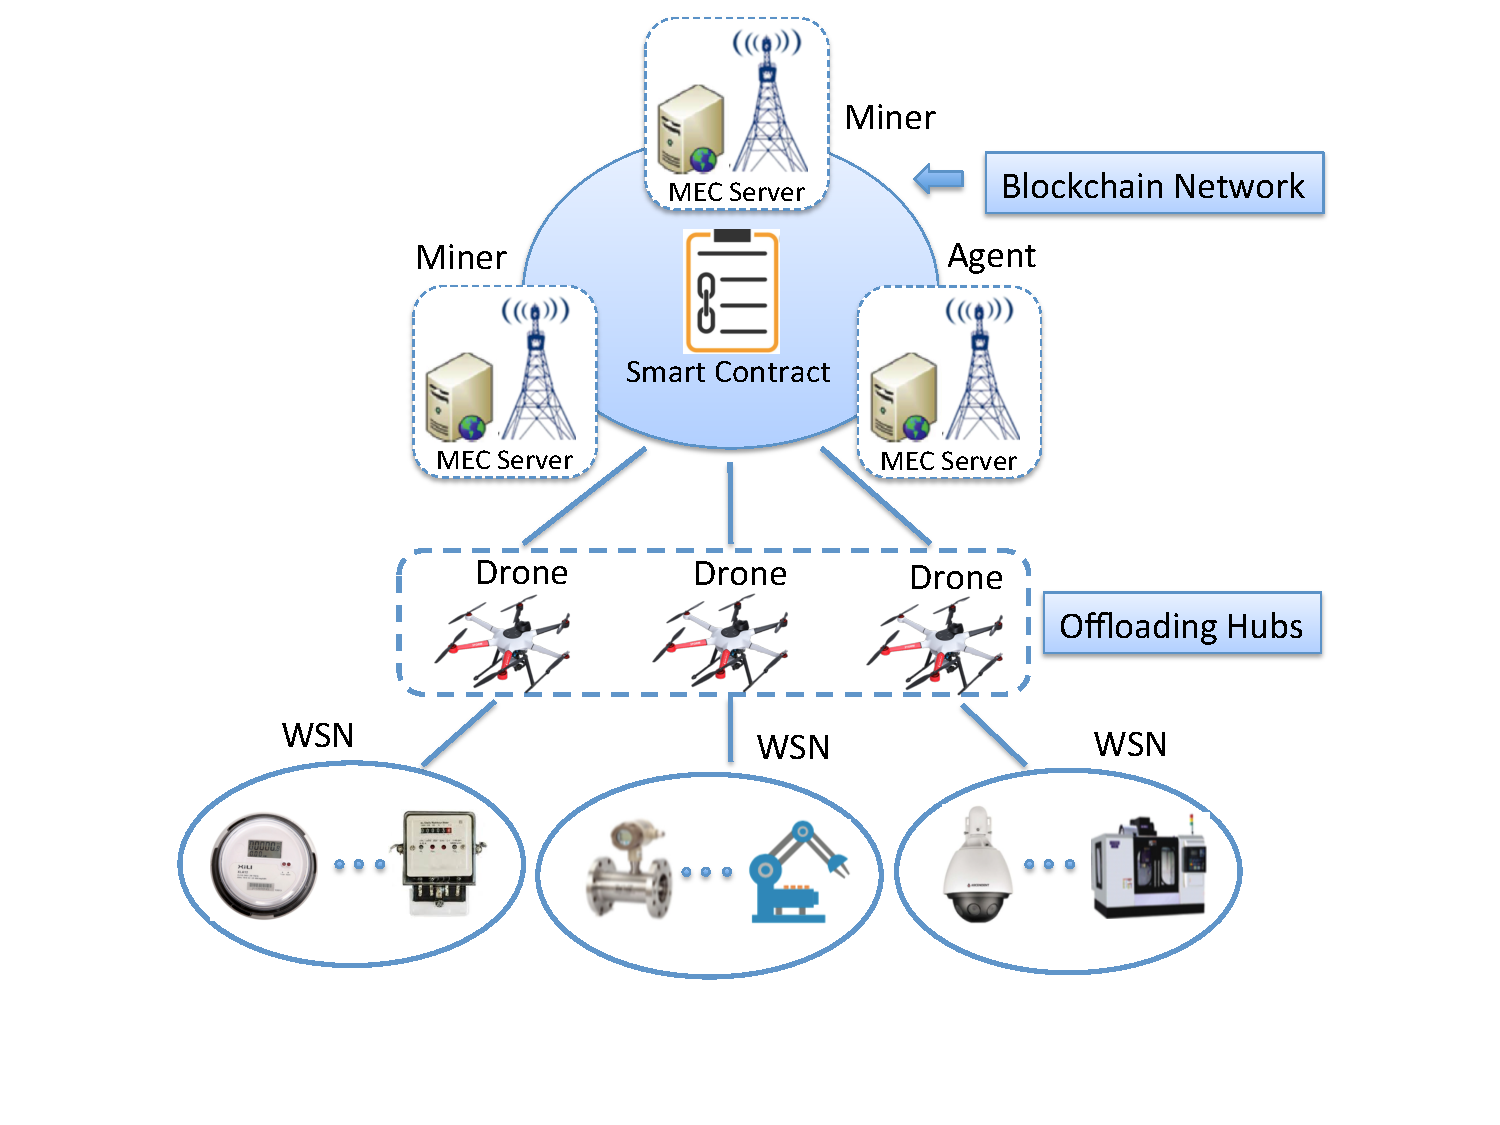
\includegraphics[width=3.5 in]{Fig/Architecture.pdf}
% \caption{Decentralized Offloading System}
% \label{fig:network-arch}
% \vspace*{-0.5\baselineskip}
% \end{figure*}



\begin{figure*}[t]
\centering
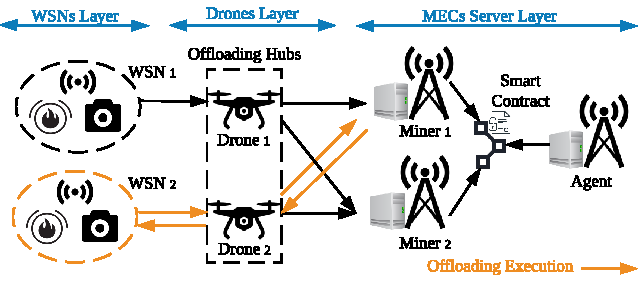
\includegraphics[width=5 in]{Fig/Architecture_1.pdf}
\caption{Decentralized Offloading System}
\label{fig:network-arch}
\vspace*{-0.5\baselineskip}
\end{figure*}


\section{Related Work}\label{sec:related_work}
The contribution of this work lies in the collaborative combination of three important cutting-edge technologies, that is offloading in MEC, UAV and blockchain. 
This section explores the previous research carried out by combining two of those technologies.

\subsection{Offloading in MEC and Blockchain}
Amounts of existing research \cite{qiu2019online,chen2019cooperative,jiang2019hierarchical} focus on offloading the blockchain mining tasks from IoT devices to the MEC servers.
Chen. et al\cite{chen2019cooperative} extended the offloading process to multi-hop network. 
Jiang. et al\cite{jiang2019hierarchical} considered two scenarios with both fixed and dynamic number of miners by formulating a multi-leader multi-follower Stackelberg game.
\cite{xu2019become} exploited using blockchain to ensure data integrity, while ignoring other security threats.
\cite{zhang2019joint} designed two smart contracts to trade the computing resource and loan coin for mobile equipment.
%\cite{seng2019d2d} concentrated on the matching between offloading tasks and the edge servers  or user equipments based on the blockchain platform.
\cite{guo2019adaptive} presented a blockchain-based MEC framework for adaptive resource allocation and computation offloading where the blockchain is responsible for the management and control functions.
However, when above frameworks of block-chain-empowered MEC integrate blockchain technology into IoT devices, they fail to consider the resource-constrained IoT devices for supporting the computation-consuming blockchain mining tasks.
% Even though there exist solutions that do not keep the entire blockchain information locally.
Our architecture avoids the mining burden of IoT devices and increases the flexibility for applications in a large scale of IoT device scenarios.

\subsection{Offloading in MEC and UAV}
UAVs feature broader communication coverage and are thus considered as relaying services providing computation offloading for mobile users in MEC scenarios \cite{jeong2017mobile}.
% considered the UAVs as means to provide enhanced coverage or relaying services to mobile users for computation offloading in MEC scenarios.
Also, the UAV's trajectory can be optimized minimizing the overall energy consumption.
% In the meanwhile, it provides the UAV’s trajectory with the goal of energy consumption minimization.
\cite{zhou2018uav} presented an UAV-aided mobile edge computing (UMEC) model, where an UAV with certain computing power is leveraged to relieve the communication and computing burden on the edge clouds.
\cite{wang2020agent} considered computation offloading to both UAV and MEC. 
The UAV agent perceives and intelligently minimizes task execution latency as well as the energy consumption.
% , the offloading system can deliver an optimum solution with minimum task execution delay and energy consumption.
UAVs are highly flexible, operable and response-sensitive. The above research works took advantages of these features, but failed to address the security challenges of UAVs.
% The above research work took advantages of UAVs including high flexibility, fast response and strong operability, but failed to address the security challenges of UAVs.
We benefit from the smart contract and give specific design for tackling the potential threats in UAVs.
% Our solution gives a specific design of the smart contract to tackle the potential threats brought by UAVs.

\subsection{UAV and Blockchain}
% \cite{lei2019securing} addressed the content poisoning problems in Named Data Networking (NDN) using UAVs. They integrated the interest-key-content binding, forwarding strategy and on-demand verification for discovering poisoned content.
\cite{lei2019securing} addressed the poisoned content discovery problems in Named Data Networking (NDN) using UAVs. They integrated the interest-key-content binding, forwarding policy and on-demand verification together to discover poisoned content.
In order to reduce the high overheads in hierarchical networks, \cite{sharma2019neural} used UAVs as on-demand nodes and presented a novel 
% neural-blockchain-based
drone-caching framework to ensure ultra-reliable communications.
The above methods are not very practical, which requires the cooperation of three blockchain. In our design, the UAV is apart from blockchain network, only playing the role of offloading hubs. The blockchain network is used to improve the users' trust for MEC service providers.
\section{System Architecture} \label{sec:arch}
In this section, we describe the architecture of the decentralized offloading system in detail.
\bin{
The architecture is composed of three layers with the flow of the data: \textit{Wireless Sensor Networks (WSNs)} layer, \textit{Drones} layer and \textit{MEC Servers} layer.
\textit{WSNs} are data generators usually deployed across various environments such as buildings, streets and forests.
The collected data is used for applications like smart building, intelligent transportation and fire alarm system etc.
\textit{Drones} layer acts as the offloading hub for catching and forwarding the data from the WSNs to the MEC servers where data processing task proceeds.} 
The processing tasks are offloaded to the ``best'' MEC server with the minimum task latency.
Finally, in \textit{MEC Servers} layer, a closed blockchain is set up among MEC servers for auditing service provider's honest during user data operation.


% The architecture is composed of three layers from the bottom to the top: Wireless Sensor Networks (WSNs) layer, Drones layer and MEC Servers layer.
% WSNs are deployed in buildings for smart building applications, in streets for intelligent transportation and in forests for fire auto-protection system, etc.
% Drone layer, namely offloading hub, that catches the data from IoT devices and forwards to MEC servers for processing. 
% The processing tasks are offloaded to the “best” MEC server with the minimum task latency.
% Moreover, the amount the MEC servers we setup a closed blockchain for auditing service provider's honest of operating users' data.




% The IoT devices in WSNs usually generate mission-critical tasks such as face recognition, which requires large computation capacity to operate and the prompt response.
% The IoT devices do not have sufficient computation resources to execute those tasks and adopt the offloading policy to help.
% In order to improve the access coverage of MEC servers without compromising the high cost of MEC servers increase, we introduce the drone layer as a offloading hub to relay and cache data from IoT devices for MEC servers.
% The offloading tasks are offloaded to the “best” MEC server with the minimum task latency.
% Due to the heterogeneous MEC servers provided by various companies, we exploit the blockchain technology to guarantee the security and visibility of the offloaded data. 
% describe the current UAV-aided scenarios
%Due to the features of high mobility and reduced infrastructure costs, drones have received wide attention in various applications\cite{wang2020agent}.
%An UAV wandering in a certain area are used as a relay to help IoT devices to offload their computing tasks to MEC servers.

\bin{
Figure \ref{fig:network-arch} illustrates the architecture of the decentralized offloading system with an example to explain the implementation details.
As shown by the orange line, $WSN_{2}$ generates a task and forward it to $Drone_{2}$. 
Next in the $Drone_{2}$ offloading hub, the smart contract decides that the task is offloaded to $Miner_{1}$ for analysis and proceeds accordingly.
After the computation is finished, the results is sent all the way back to the original location where the data is generated. 
We explain the main components for each layer that jointly execute the aforementioned example:
\begin{itemize}
\item Wireless Sensor Networks (WSNs) layer:
This layer usually contains multiple IoT sensors collecting data from physical environment for various IoT applications. 
The IoT devices within WSNs usually have limited computational power, memory and energy storage which necessitates the offloading operation.
\item Offloading Hubs (Drones layer):
 In our architecture, a drone is used as an offloading hub and is  responsible for: 1) relaying the offloading tasks to an appropriate MEC server, 2) translating the inter WSNs-blockchain communication protocol.
Specifically, all drone and MEC servers are interconnected, with each drone receiving data from multiple WSNs (IoT devices)
IoT devices will only be able to request offloading information from the blockchain using the offloading hub.
\item Blockchain network (\textit{MEC Servers} layer):
In the \textit{MEC Servers} layer, a blockchain network is deployed with a smart contract committing data offloading policy.
The blockchain network contains two types of nodes: the \textit{Agent} and the \textit{Miner}.
The \textit{Agent} is responsible for generating and deploying the smart contract to the blockchain network, such that each node in the blockchain can execute the smart contract automatically.
The offloading tasks are then assigned to smart contract qualified \textit{Miner} nodes. 
All operations from the assigned \textit{Miner} are recorded to blockchain for further verification.
The blockchain network in our architecture is designed as a private blockchain for its specific functionality. 
We chose a private blockchain since it has extra access limitation for participators to guarantee the authority of MEC servers.
%However, in a real scenario, a public blockchain should be used to facilitate the adoption of the solution.
\end{itemize}
}

% Figure \ref{fig:network-arch} illustrates the decentralized offloading system with the blockchain network, where a smart contract with committed offloading policy is deployed in MEC servers. 
% The blockchain network contains two types of nodes: the agent and the miner.
% The agent is responsible for generating the smart contract and deploying it to the blockchain network, such that each node in the blockchain can execute the smart contract automatically.
% If a miner is qualified by the smart contract, the offloading task can be assigned. All operations from the assigned miner will be recorded to blockchain for further verification.
% The main components in this architecture are illustrated as follows.
% \begin{itemize}
% \item Wireless Sensor Networks (WSNs):
% This layer is used to collect data from physical environment for various IoT applications. 
% Besides, the IoT devices within WSNs usually have limited computational power, memory and energy storage.
% \item Offloading Hubs:
%  In our architecture, a drone is used as an offloading hub, which is responsible for relaying the offloading tasks to an appropriate MEC server, as well as translating the communication protocols among WSNs and the blockchain network.
%   The drone is connected directly with a MEC server. 
%  Multiple WSNs can be connected to a drone and an IoT device can be connected to several drones which is convenient for handover.
%  Moreover, multiple drones can be connected to the same MEC server.
%   IoT devices will only be able to request offloading information from the blockchain using the offloading hub.
% \item Blockchain network:
% The blockchain network in our architecture is designed as a private blockchain for its specific functionality. 
% We chose a private blockchain since it has the extra access limitation for participators to guarantee the authority of MEC servers.
% %However, in a real scenario, a public blockchain should be used to facilitate the adoption of the solution.
% \end{itemize}






\section{System design}\label{sec:sys}
This section gives a depiction of the operations designed in the smart contract and the interaction procedure between the components of our architecture. Moreover, we give some discussion about the system limitations. 
 
\subsection{Smart Contract}
Figure \ref{fig:data-structure} shows the data structure in the smart contract.
Each drone covers one or multiple WSNs and takes responsibility for a set of IoT devices in the WSNs, and each IoT device generates at most one offloading task at one time.
The task will be offloaded to a specific MEC server by smart contract through a drone.

It is assumed that $I$ is the set of public keys of $I(d)$ of each drone $d$, 
$G$ is the set of the public keys $G(m)$ of each IoT device $m$ and $P$ is the set of offloading policies where $p$ refers to the specific offloading rules to select the ``best" MEC server to offload tasks from IoT devices.
%$$I=\{I(d_1),I(d_2),...,I(d_n)\}$$
%$$G=\{G(m_1),G(m_2),...,G(m_n)\}$$
%$$Q=\{Q(s_1),Q(s_2),...,Q(s_n)\}$$
%$$P=\{p_1,p_2,...,p_n\}$$


\begin{figure}[t]
\centering
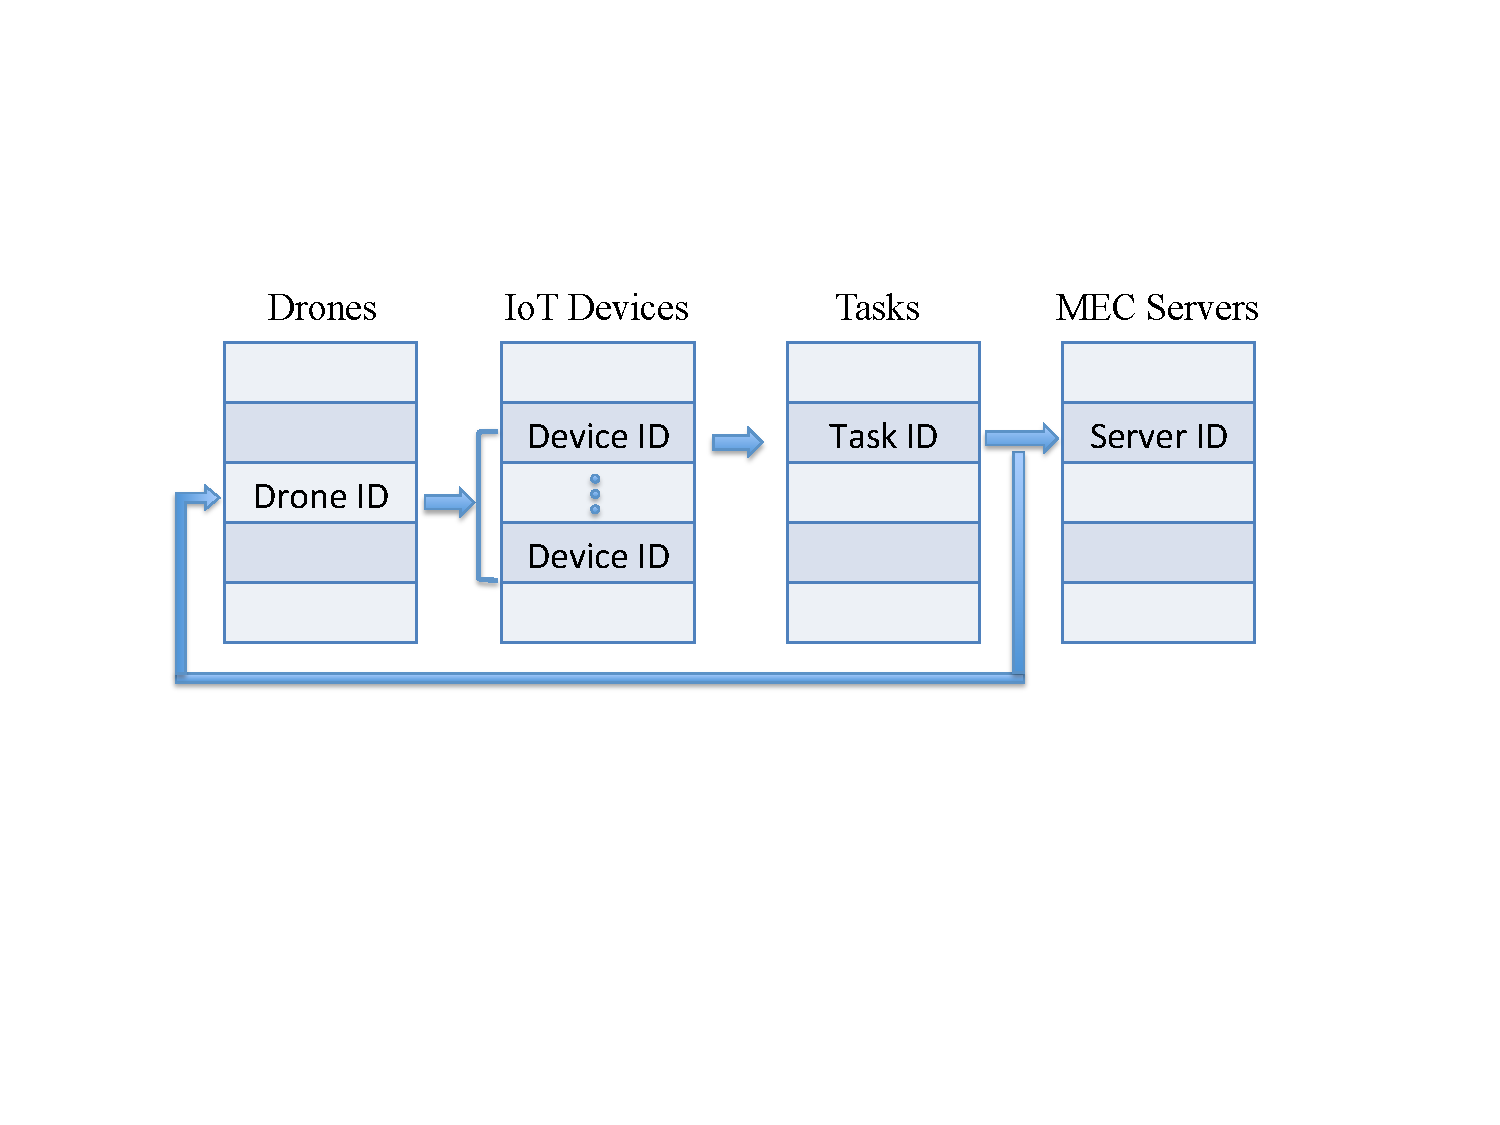
\includegraphics[width=3.3 in]{Fig/DataStructure.pdf}
\caption{Data Structure in the Smart Contract}
\label{fig:data-structure}
\end{figure}

In the smart contract,  the drones and IoT devices are identified in the offloading system by their public keys.
The order of components registration is depicted below.
First MEC servers are signed in by the operation $RegisterServer(Q(s))$, next the drones are joined by  $RegisterDrone(Q(s), I(d))$ iff drone $d$ is authorized by MEC server $s$.
After that, the IoT devices are registered by $RegisterDevice(I(d), G(m))$ iff drone $d$ is the offloading hub of device $m$. 
Besides, the tasks will be identified by their IDs.
The mapping from the drone to the IoT device is done by $AddDronetoDevice(I(d), G(m), Q(s), p)$ iff drone $d$ is the offloading hub of device $m$.
The offloading policy can be deployed into the smart contract by $AddOffloadingPolicy(I(d), G(m), Q(s), p)$, which determines how to choose the MEC server to offload.
When it needs to find the offloading hub of the specific IoT device, $QueryDrone(I(d))$ can be called.
$QueryOffloading(I(d), t, G(m), Q(s), p)$ is used to obtain the result of offloading task $t$ by executing offloading policy $p$.
It is worthy to mention that the fetching process does not incur any fee or latency, since drones obtain the information from the blockchain store directly, rather than use a transaction. 

% The operations defined in our smart contract are described as follows.
% \begin{itemize}
%\item $RegisterServer(Q(s))$: $Q^* \leftarrow Q \bigcup Q(s)$ for any MEC server $s$.
%\item $RegisterDrone(Q(s), I(d))$: $I^* \leftarrow I \bigcup I(d)$ iff drone $d$ is authorized by MEC server $s$.
%\item $RegisterDevice(I(d), G(m))$: $G^* \leftarrow G \bigcup G(m)$ iff drone $d$ is the offloading hub of device $m$. 
%\item $AddDronetoDevice(I(d), G(m))$: $G^* \leftarrow G \bigcup G(m)$ iff drone $d$ is the offloading hub of device $m$.
%\item $AddOffloadingPolicy(I(d), G(m), Q(s), p)$: $P^* \leftarrow P \bigcup p$ iff drone $d$ is the offloading hub of device $m$.
%\item $DeRegisterServer(Q(s))$: $Q^* \leftarrow Q \bigcap Q(s)$.
%\item $DeRegisterDrone(I(d))$: $I^* \leftarrow I \bigcap I(d)$.
%\item $DeRegisterDevice(G(m))$: $G^* \leftarrow G \bigcap G(m)$.
%\item $QueryDrone(I(d))$: returns the tuple $(d,U)$ where $U=\{u \in G, d$ is the offloading hub of device $u\}$. 
%\item $QueryOffloading(I(d), t, G(m), Q(s), p)$: returns the result of offloading task $t$ by executing offloading policy $p$.
%\end{itemize}


\subsection{Offloading Policy}
The offloading policy plays a crucial part as it determines which local MEC server would be performed the offloading computation task.
Currently, the design of offloading policies usually takes multiple factors into consideration together, such as the distance of the request device and the MEC server, the access and computation capacity of MEC servers, the security level of MEC servers, and the availability of wireless connection links, etc.
In this paper, we only consider some simple offloading policies as discussed in the following.

\subsubsection{The Random Policy}
When the drone has no prior knowledge about the MEC servers, the drone will choose randomly one MEC server to offload the task delivered from IoT devices.

\subsubsection{The Nearest Policy}
The drone will connect with the nearest available MEC server in the blockchain network, a miner node in Figure \ref{fig:network-arch}.
The nearest policy indicates that drones always find the nearest MEC server to offload the task from IoT devices.

\subsubsection{The Max Computing Capacity (MCC) Policy}
In max computing capacity policy, the drones always choose the MEC server with the maximum computing capacity to offload tasks.

\subsubsection{Smart Contract Policy}
 In our smart contract policy, it aims to find the best offloading MEC server with minimum latency.
 Since the scale of the blockchain network is so small, we assume that the consensus time is negligible or with little difference among different policies.
 Thus, we focus on the task transmission delay and computation offloading delay.
Given that $a_t$ is the data amount of offloading task $t$, $\bar{r}$ the average transmission rate, $b_t$ is the computation amount of offloading task and $\bar{c}$ the average computing capacity, the drone will choose the MEC server by the Nearest policy if $a_t/\bar{r}   >  b_t/\bar{c}$, otherwise by the MCC policy.




 
\subsection{System Interactions}
Figure \ref{fig:SmartContract} illustrates the interactions among the system components, which can be divided into three phases: establishing the blockchain network, signing the drones and IoT devices into the system, and executing the offloading operation for the tasks from IoT devices.

\begin{figure*}[t]
\centering
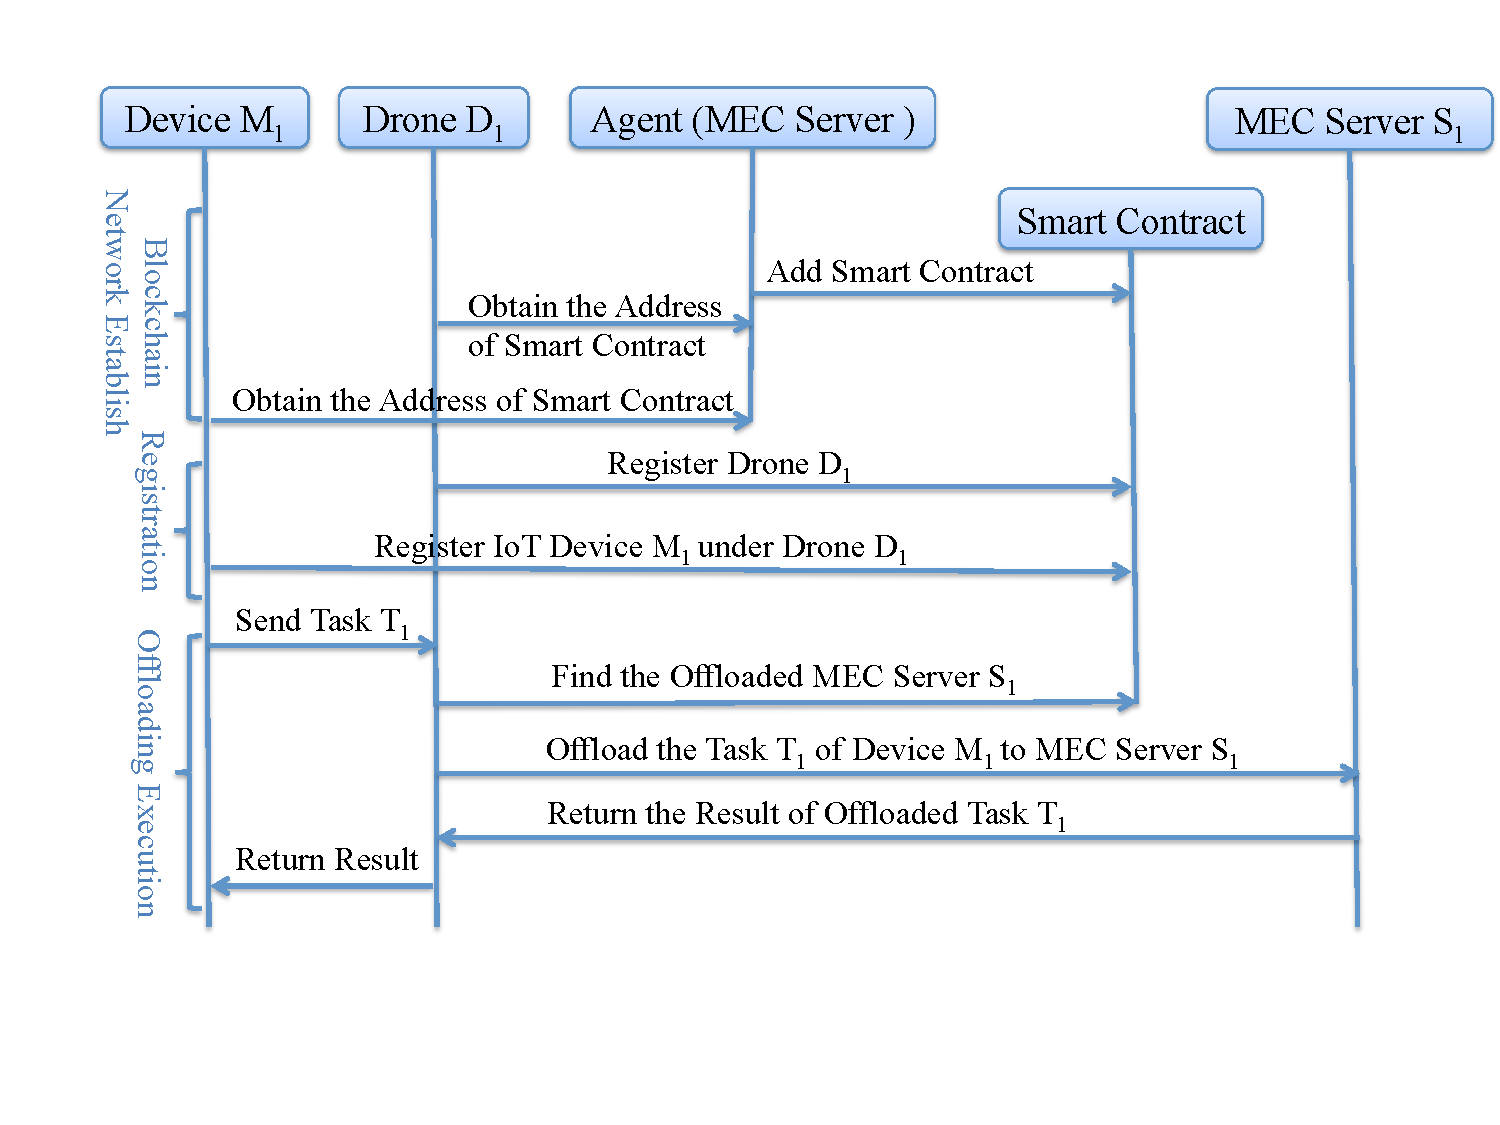
\includegraphics[width=4.5 in]{Fig/SmartContract.pdf}
\caption{Network Establishment, Registration and Offloading Execution}
\label{fig:SmartContract}
\end{figure*}

\subsubsection{Network Establishment}
 The blockchain network is established among the network of MEC servers in the beginning. 
Once the blockchain network is created, the agent node takes the responsibility to deploy the smart contract into the blockchain network. 
The smart contract defines all the operations of the offloading policy and it will generate an unique address to identify this smart contract when it is accepted by the blockchain network.
All components in the offloading system use that unique address to interact with the smart contract and execute the operations automatically designed in the smart contract.
 For example, all the drones in the system need to register as offloading hubs by interacting with the smart contract.

Figure \ref{fig:SmartContract}  shows how a drone interact with the address and query the Agent node. 
The offloading hub connects with several available MEC servers in the blockchain network, i.e., miner nodes.
 Each miner hosts a distributed copy of the blockchain to make all the operations to offloaded data accountable.

\subsubsection{Registration}
 Any MEC server in the offloading system can be registered into the blockchain network. 
Before a drone is registered as a offloading hub, it needs to be authorized by the node of the blockchain network.
 Then it registers to the blockchain network by interacting with the smart contract. 
 After then, the IoT devices can be registered by the registered drones thought the address of the smart contract.
 Meanwhile, drones  will receive an address of the registered device to identify who is the offloading hub of the device.
 The $QueryDrone()$ operation can verify the registration of IoT devices under a drone.



\subsubsection{Offloading Execution}
After the IoT devices and drones are signed into the specific smart contract, the offloading policy is executed automatically for task $T_1$ of device $M_1$.
The IoT device $M_1$ first sends the offloading task to its offloading hub, a verified drone, then the drone transfers the data and execution tasks to the selected MEC server for offloading.
The MEC server selection is based on the offloading policy in the smart contract.
All the processing or operation to users' data as long as the execution results will be publish to the blockchain network. At the same time, the execution results will be sent to the drone and forwarded back to IoT device $M_1$.


\subsection{Tackle of Blockchain's Limitations}
In this subsection, we illustrate how our propose system to overcome the limitations of blockchain systems.

\subsubsection{Cryptocurrency Fees}
In the blockchain platform, the cryptocurrency fees are used to award the miners who successfully manage their mined blocks into the blockchain for all transactions.
It is also required a minimum fee for a transaction in some public ledgers to avoid spam transactions. In our case, this fee is covered on users' services fee. All MEC servers are motivated to mine the blockchain. 

\subsubsection{Consensus time}
It is well known that the consensus procedure in blockchain occupies the most time during a transaction generation.
However, in our system the number of MEC server is limited in a private blockchain, thereby significantly reducing the consensus time. If we wait for a offloading task's results writing into blockchain before sending them back to corresponding IoT device, it still introduce huge delay. Therefore, in our design that obtained results can be returned immediately and must be returned by the drone which signs the smart contract. As a result, we solve the delay issue and also prevent the threat that unauthorized drone steal the offloading information.     

% However, the drone do not use transactions to request information from the blockchain network in our solution. 
% Hence, the drone can query information immediately from the connected node of blockchain network. 
% In the meantime, the drone can response for the requests of IoT devices in real time.
% In addition, transactions created by the MEC server may incur long delay, which might brings new potential threat.
% For example, an unauthorized attacker (MEC server) could obtain the offloading information before the revoked operation by the MEC server is spread and accepted by the majority of the miners.
% In our solution, the offloading policy designed in the smart contract is easily to obtain the result, which makes the MEC server can response the request from the drone in real time and tell it which MEC server to offload.
\section{Security Analysis}\label{sec:security_analysis}
% subsequently shed light on a variety of potential security threats and the possible solutions.

Security is essential for any management systems, and our offloading system is of no exception. 
% The design of our system aims to facilitate the offloading in constrained scenarios, as well as provide a security guarantee. 
In this section, we identify main threats in our proposed architecture. After that, some solutions are proposed to deal with the threats. 

To this end, we use the STRIDE thread model\cite{hernan2006threat} as the security criteria which has six categories: \textbf{S}poofing, \textbf{T}ampering, \textbf{R}epudiation, \textbf{I}nformation disclosure, \textbf{D}enial of service(DoS), and \textbf{E}levation of privilege. Table \ref{tab:threat-property} shows the relations between the threats and the security properties of a system.

\begin{table*}[htbp]
\caption{Threats and Security Properties}
\begin{center}
\begin{tabular}{|p{85pt}||p{65pt}|p{200pt}|}
\hline
Threat & Property & Description \\
\hline
\textbf{S}poofing & Authentication & The identity of users is established.\\
\textbf{T}ampering & Integrity & Data can only be modified by verified person.\\
\textbf{R}epudiation & Non-repudiation & Not denial actions are allowed.\\
\textbf{I}nformation disclosure & Confidentiality & Control the access to the data.\\
\textbf{D}enial of service & Availability  & System is ready for receiving tasks.\\
\textbf{E}levation of privilege & Authorization & Identify the users who can access the data. \\
\hline
\end{tabular}
\label{tab:threat-property}
\end{center}
\end{table*}

Based the model, we list the security threats of our system in Figure \ref{fig:security-analysis} and propose some prevention solutions in the following.
% As shown in Figure \ref{fig:security-analysis}, some components in our system is still susceptible to some security threats.
 \begin{itemize}
\item MEC Server: Overall, the blockchain guarantees the security of MEC servers, specifically, the data integrity and availability.
The authentication process of the blockchain ensures that MEC servers never disclose offloading information. 
In addition, the traceability property of the blockchian prevents the MEC servers from tampering the results of offloading tasks or repudiating their actions.
\item Drone: A malicious drone could spoof (impersonate a normal offloading hub), tamer (change the offloading information during data transmission), repudiate (deny performing an action), DoS (degrade the relay service to IoT devices) or disclose sensitive information of IoT devices.
Signature certification could solve the above potential threats.
Drones could get signed certificates from a MEC server from the blockchain network, and IoT devices could verify the authentication of the offloading hub by those certificates.
\item IoT device: If a trust device is impersonated by a malicious IoT device, it may spread poison content into the offloading system, which consumes the network resources and has a great impact on the performance of task offloading.
The authentication of IoT devices can also avoid the above security threats. 
% Once an IoT device is registered in the system, the drone who manages its offloading request could authenticate its identity.
\end{itemize}


\begin{figure}[t]
\centering
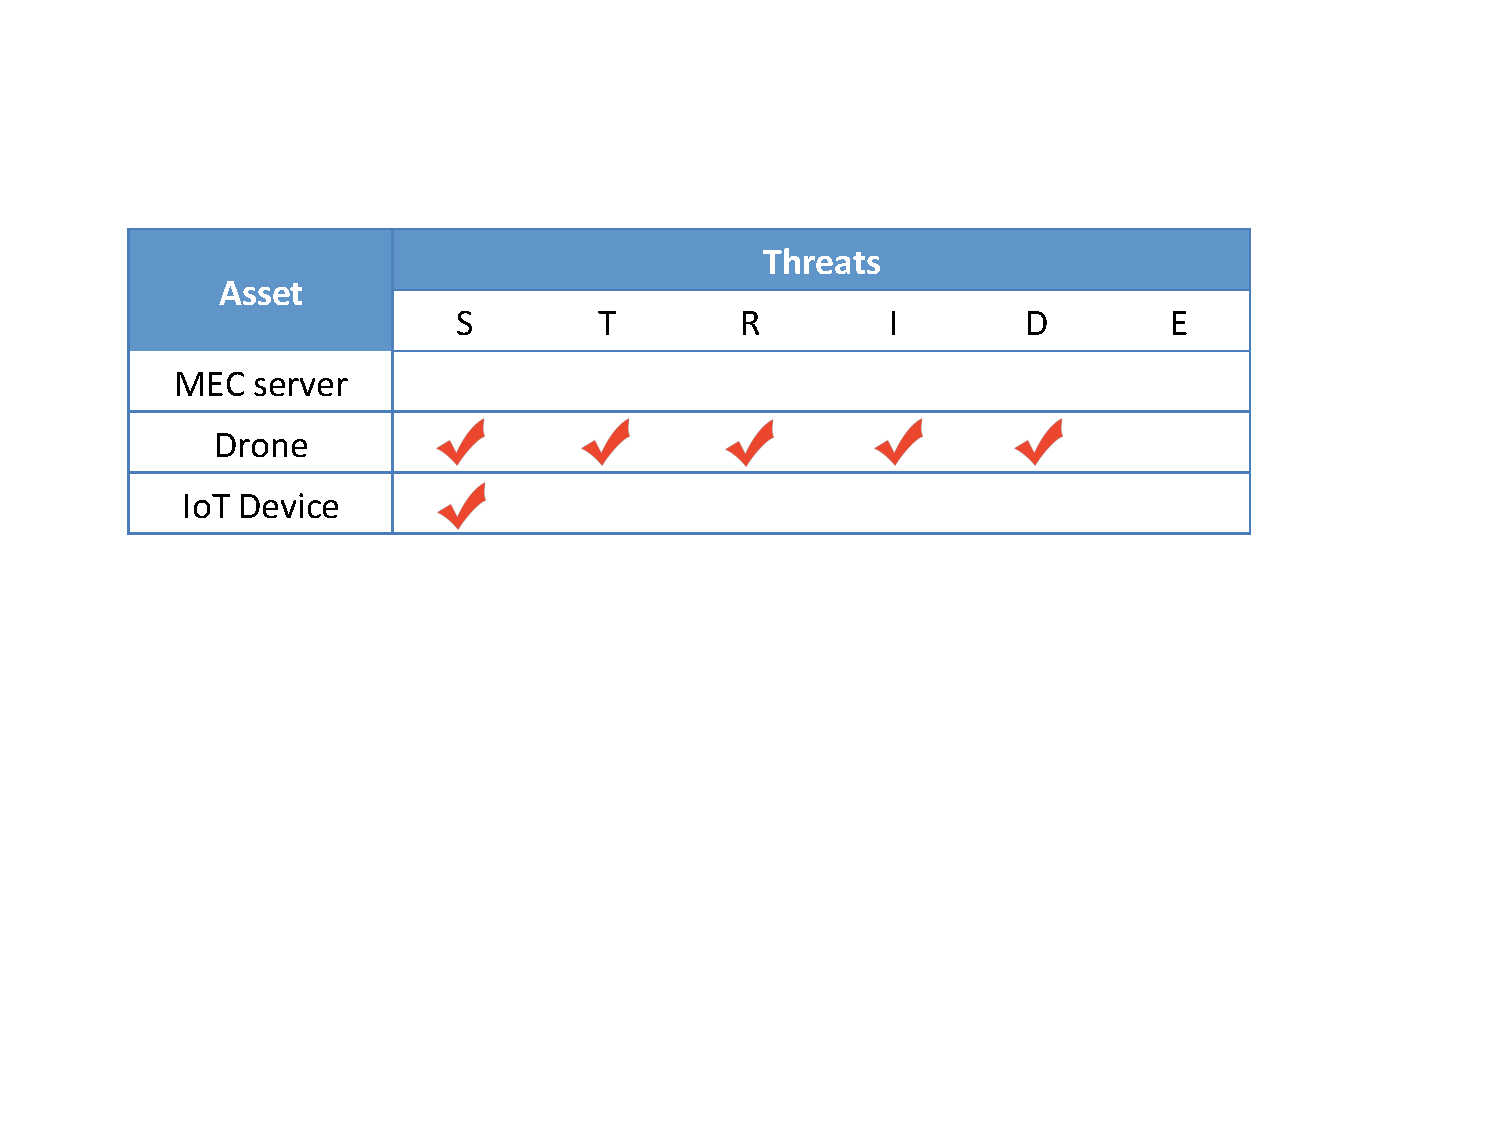
\includegraphics[width=3.3 in]{Fig/SecurityAnalysis.pdf}
\caption{Potential Security Threats}
\label{fig:security-analysis}
\end{figure}

\section{Performance Evaluation}\label{sec:eva}
In this section, we aim to evaluate the feasibility of the proposed architecture which is suitable for any off-loading policy.

\noindent \textbf{Experiment setup.} We implemented the contract in Solidity 0.4.26 \footnote{https://solidity.readthedocs.io/en/v0.4.24/} on the test net of Ethereum network, “Ropsten \footnote{https://ropsten.etherscan.io/}”, which is a popular blockchain test net for evaluation of smart contracts.
Moreover, we emulate a scenario that one drone carries a set of tasks to be offloaded to three MEC servers. 
Four policies discussed in section 3.2 are developed in our smart contract and are used to generate offloading solutions for the submitted tasks.
% For simplicity, we generate four accounts on “Ropsten” to simulate two roles: the drone and MEC servers, where one for the drone and three for MEC servers.

% Since the communication between WSNs and drones is not belonged to the smart contract, we have not implemented that part in our experiment.
% The smart contract focuses on MEC server selection for drones with different offloading policies.
% The smart contract includes four simple offloading policies introduced in section 3.2, the Random policy, the Nearest policy, the MCC policy and the DelayAware policy.
% In our experiment, the account simulated the drone is responsible for the publish of the smart contract, and the other accounts register to the smart contract.
% All registered accounts can communicate with the interfaces to capture or transmit the related information.

In our smart contract, we define an interface $GetTaskInfo()$ to capture the task information, including data amount, computation amount and ID, meanwhile anther interface $GetServerInfo()$ is defined to obtain the MEC server information, such as MEC-Drone distance, computation capacity and address.
% In order to compare the cost of various offloading policies, we define four interfaces to conduct the corresponding policies, i.e., the random policy, the nearest policy, the MCC policy and the DealyAware policy.

\noindent \textbf{Evaluation metrics.}
We measure the performance of the policies via ``Gas'' which is the cost for the miners to execute the transactions. This cost depends on the complexity of each policies, i.e., how much computation and storage resources are consumed for running the smart contract. Each experiment is repeated 20 times, and the average values and their variance are reported.

% The complexity of each interface in the smart contract depends on the its required computation and storage resource.
% Since the interface needs the miner to invoke, more payment to the miner is required with more complex interface to  be executed.
% The payment to the miner is called the transaction fee, measured as “Gas” defined in Ethereum, which is a unit to evaluate the miner‘s work amount when it executes the transaction.
% Hence, we record the gas consumption of each interface with the increase number of offloading tasks. 


Figure \ref{fig:Gas} demonstrates the experimental results, where the DelayAware policy consumes more gas than others with the increasing number of tasks.
For convenience of analysis, the number of offloading tasks is assumed as $n$, while the number of MEC servers is represented as $m$.
The reason is that the time complexity of the DealyAware policy is $O(2n+m)$, relatively simpler than other policies, i.e., the random policy is in $O(n)$ time, the Nearest policy and MCC policy are the same with the time complexity of $O(n+m)$.
In this experiment, $m$ is a constant, equal to 3.
Hence, the gas consumption of all four policies is linearly increasing with the number of offloading tasks.

\begin{figure}[t]
\centering
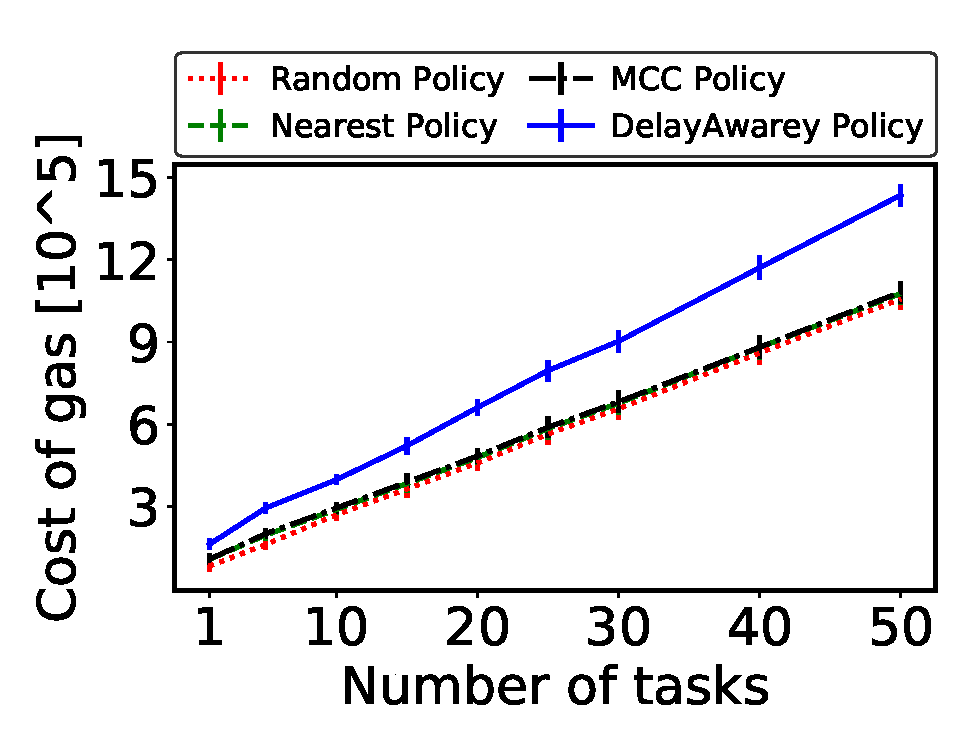
\includegraphics[width=3in]{Fig/PolicyGas.pdf}
\caption{The Gas Consumption under Different Offloading Policies}
\label{fig:Gas}
\end{figure}


\section{Conclusion and Future Work}
In this paper, we present a novel architecture for automatically distributed offloading systems in droned-based MEC scenarios.
The architecture brings in the drone as the offloading hub to detect the authorized IoT devices and help them to offload tasks to MEC servers based on the blockchain technology.
The architecture supports the mobility of IoT devices and allow them to join or leave at any time.
To evaluate the system performance, we focus on the offloading latency introduced by the smart contract, and the results demonstrate that the high reliable offloading policy deployed on the smart contract is feasible in specific scalable MEC scenarios.

Our future work focuses on two parts:
\begin{enumerate}
\item Establish a real private blockchain network to evaluate the practical performances, such as the latency and overhead of smart contracts.
\item Design more intelligent offloading policy to apply for more complex scenarios, such as the drones have high mobility to collect the data from IoT devices.
\end{enumerate}




\ifCLASSOPTIONcaptionsoff
  \newpage
\fi




\bibliographystyle{IEEEtran}
\bibliography{myRef}

\vskip -2\baselineskip plus -1fil
\begin{IEEEbiographynophoto}{Shuyun Luo}{\,}is a lecture at Zhejiang Sci-Tech University, China. 
Her research interests include edge computing, reinforcement learning and network economics.
Email: shuyunluo@zstu.edu.cn
\end{IEEEbiographynophoto}
\vskip -2\baselineskip plus -1fil
\begin{IEEEbiographynophoto}{Hang Li}{\,}is a master student at Zhejiang Sci-Tech University, China.
His research interests include UAV-based edge computing. 
Email: zstlihang@163.com
\end{IEEEbiographynophoto}
\vskip -2\baselineskip plus -1fil
\begin{IEEEbiographynophoto}{Zhenyu Wen}{\,}is currently a postdoc researcher with the School of Computing, the Newcastle University, UK.
His research interests include Multi-objects optimization, Crowdsources, AI and Cloud computing.
Email: Zhenyu.Wen@newcastle.ac.uk
\end{IEEEbiographynophoto}
\vskip -2\baselineskip plus -1fil
\begin{IEEEbiographynophoto}{Bin Qian}{\,}is a postgraduate research student in the school of computing, Newcastle University, UK.
His research interests include IoT, Machine Learning. 
Email: b.qian3@ncl.ac.uk
\end{IEEEbiographynophoto}
\vskip -2\baselineskip plus -1fil
\begin{IEEEbiographynophoto}{Graham Morgan}{\,} is a reader in the School of Computing, Newcastle University. Area of expertise: Cloud Computing, Video Games, Distributed Systems, Deep Learning
Email: graham.morgan@ncl.ac.uk
\end{IEEEbiographynophoto}
\vskip -2\baselineskip plus -1fil
\begin{IEEEbiographynophoto}{Omer Rana}{\,}is a full professor of performance engineering in the School of Computer Science and Informatics at Cardiff University. His research interests include performance modelling, simulation, IoT, and edge
analytics. Contact him at ranaof@cardiff.ac.uk. 
\end{IEEEbiographynophoto}
\vskip -2\baselineskip plus -1fil
\begin{IEEEbiographynophoto}{Rajiv Ranjan}{\,}is a Chair and Professor at Newcastle University, UK, and at China University of Geosciences, China.
He has expertise in cloud computing, big data, and the Internet of Things.
Email: raj.ranjan@ncl.ac.uk
\end{IEEEbiographynophoto}



\end{document}


